% ---------------------------------------------------
%
% Trabajo de Fin de Grado. 
% Author: Laura Padrón Jorge. 
% Capítulo: Tecnologías utilizadas en el Trabajo de Fin de Grado. 
% Fichero: Cap3_Technology.tex
%
% ----------------------------------------------------
%

\cleardoublepage
\chapter{Tecnologías} \label{chap:polytopes} %Cambiar por el label adecuado. 

En este capítulo se habla de las principales tecnologías que han sido utilizadas durante la elaboración de este TFG.

\section{Beacons}

\textit{''Beacons''} \cite{URL::Beacons} cuya traducción del inglés equivaldría a \textit{''balizas''} o \textit{''faros''}, es una tecnología emergente que desde algunos años se está intentando abrir paso en el mercado. Como su propio nombre indica, estos dispositivos intentan dar una mejor solución al posicionamiento en interiores, siendo un mecanismo de guía en lugares donde otras tecnologías, como el GPS o el Wifi dejan de funcionar o resultan imprecisas. 


Sin embargo, estos no son los únicos usos de los beacons, actualmente muchas empresas están ampliando sus usos a otros campos, y el diseño de estos beacons se está presentando en tamaños tan pequeños y con un tiempo de funcionamiento tan elevado, que se pueden desplegar prácticamente en cualquier lugar sin dificultades.

%\begin{figure}[h]
%	\left
%	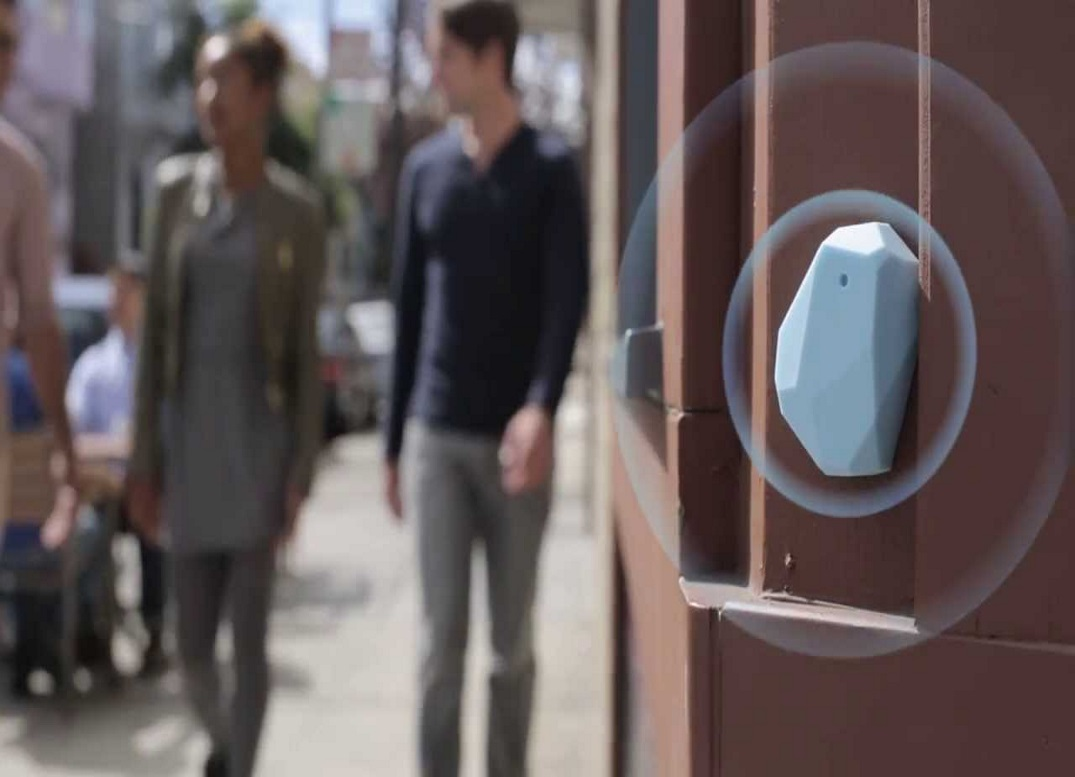
\includegraphics[width=\columnwidth]{estimoteBeacon.png}
%	\caption{Uno de los beacons de la compañia Estimote}
%	\label{fig:estimote_Beacon}
%\end{figure}

%\begin{figure}[h]
%	\middle
%	\includegraphics[width=\columnwidth]{estimoteBeaconSticker.png}
%	\caption{Uno de los beacons de la compañia Estimote en formato Pegatina}
%	\label{fig:estimote_Beacon_Sticker}
%\end{figure}

%\begin{figure}[h]
%	\right
%	\includegraphics[width=\columnwidth]{BluesenseBeacon.png}
%	\caption{Uno de los beacons de la compañia BlueSense}
%	\label{fig:bluesense_Beacon}
%\end{figure}

A continuación se intentará responder a las preguntas más frecuentes que nos pueden surgir con respecto a esta tecnología:


\begin{itemize}
\item ¿Qué es un Beacon?
\item ¿Cómo funcionan estos dispositivos?
\item ¿Qué rango de alcance poseen?
\item ¿Con qué dispositivos móviles son compatibles? 
\item ¿Qué ventajas y desventajas tienen con respecto a otras tecnologías?
\item ¿Qué usos se le ha dado a esta tecnología hasta ahora?
\item ¿Qué empresas trabajan con esta tecnología?
\end{itemize}

\subsection{¿Qué es un Beacon?}

Para los que no hayan oido este término, en el marco en el que nos movemos, hace referencia a un pequeño dispositivo (sus tamaños varían de uno a otro, pero siempre de tamaño reducido) que emite señales de onda corta utilizando la tecnología Bluetooth \cite{URL::Bluetooth}. Estas señales contienen una pequeña cantidad de información y son recibidas por dispositivos móviles con tecnología Bluetooth dentro de un rango de cobertura variable dependiendo del propio dipositivo. Normalmente, la fuerza de esta señal y su frecuencia son configurables.

%Foto de algo que tenga que ver con el Bluetooth 

El funcionamiento de un beacon es sencillo: El beacon emite una señal ininterrumpida que es captada por los dispositivos móviles dentro de su radio de cobertura, esta señal contiene información capaz de definir una localización, detectar y localizar otros dispositivos. A continuación la señal es captada por una aplicación movil previamente instalada, que dependiendo de la señal recibida, puede lanzar una acción en dicho dispositivo.


Hay que tener en cuenta que esta señal es unilateral: los beacons son capaces de enviar señales pero no están preparados para recibirlas. También hay que tener en cuenta, que la mayoría de las beacon actuales en el mercado transmiten información preconfigurada, confiando en la aplicacion móvil para utilizar la información; sin embargo es muy posible que esto cambie en un futuro, ampliando las posibilidades de los beacons.

\subsection{¿Como funcionan estos dispositivos?}

Los beacons usan Bluetooth Low Energy (BLE) \cite{URL::BluetoothLowEnergy}, una version del protocolo Bluetooth diseñada para usar mucha menos energía y enviar menos información. Los beacons funcionan con baterías cuyo tiempo de vida depende de la configuración establecida, teniendo en cuenta la emisión de la señal (fuerza y frencuencia) y tiempo de hibernación. Sus tiempos de vida son variables, pudiendo durar desde un mes hasta varios años. 



%Foto de una beacon de aruba por dentro con las baterías a la vista.

Independientemente de lo que se pueda pensar, los beacons en si mismas no transmiten información significativa, transmiten identificadores cortos junto con información customizable breve, que son interpretadas por una aplicación que sabe lo que tiene que hacer con esa información y que es la que se encarga de procesar la información y realizar una acción pertinente.

Este identificador se divide en tres partes: 

\begin{itemize}
\item \textit{''UUID''} \cite{URL::UUID} : corresponde con una ID dada por el vendedor e identifica el beacon en cuestión.
\item ID Superior : customizables y utilizadas con un significado específico que puede identificar una acción o parámetro. 
\item ID Inferior: customizables y utilizadas al igual que la superior con un significado específico que se puede usar para identificar una acción o parámetro.
\end{itemize}

%Imagen del numero identificativo de la Beacon.

\subsection{¿Qué rango de alcance poseen?}

Actualmente los beacons presentan un rango de aproximadamente 70 metros sin obstáculos, esta demostrado que este rango disminuye significativamente al atravesar paredes de metal o ladrillo, otros materiales disminuyen en menor medida el rango. 

Los beacons además trabajan con tres rangos de distancia principalmente: 

\begin{itemize}
\item Lejos: diseñado para que el dispositivo móvil pueda lanzar una acción cuando estás en el rango exterior de un beacon, acabas de entrar en el rango del beacon.
\item Cerca: diseñado para que el dispositivo móvil pueda lanzar una acción cuando estás en el rango interior del beacon. 
\item Inmediato: Diseñado para que el dispositivo móvil pueda lanzar una acción cuando te encuentres manejando el beacon, la posición del beacon cambia.
\end{itemize}

\subsection{¿Con qué dispositivos funcionan?}

Las beacons son compatibles con todos los dispositivos que soporten Bluetooth Low Energy, pero para que las señales de los beacons sean detectadas por tu dispositivo, se ha de tener activado el Bluetooth. 


En dispositivos con IOS7 \cite{URL::IOS7} o superior, el dispositivo puede estar constantemente buscando dispositivos BLE y despertar a las aplicaciones implicadas cuando entran en el rango de los beacons, incluso estando cerradas las aplicaciones.


En dispositivos Android \cite{URL::Android} el sistema operativo no está preparado para escanear dispositivos BLE, por lo que son las aplicaciones las que se tienen que encargar de escanear las proximidades buscando beacons, esto supone que las aplicaciones tienen que estar funcionando, despiertas (aunque sea en segundo plano).

Por último en dispositivos Windows Phone \cite{URL:WindowsPhone} o Blackberry \cite{URL:Blackberry} existen diferentes niveles de compatibilidad pero en los que soportan BLE, en funcionamiento es similar al de los dispositivos Android. 

\subsection{¿Qué ventajas y desventajas tienen con respecto a otras tecnologías?}

A la hora de hablar de los beacons existen una serie de ventajas pero también podemos encontrar algunas desventajas que iremos detallando a continuación. 


Las principales ventajas que se distinguen a la hora de hablar de las beacons son las siguientes: 

\begin{itemize}
\item A diferencia de la tecnología GPS, la activación del bluetooth consume mucho menos batería. 
\item Es una tecnología que puede ser dependiente de la red de datos. 
\item A diferencia de la tecnología GPS, sigue funcionando con gran precisión en el interior de los edificios.
\end{itemize}

En cuanto a las desventajes que nos podemos encontrar destacamos:

\begin{itemize}
\item Dependen de aplicaciones instaladas en el dispositivo móvil para funcionar. 
\item Es necesario tener el bluetooth activado, lo que consume batería en el tiempo. 
\item Su utilidad depdende de la voluntad de terceros de utilizar estos dispositivos, configurarlos y distribuir las aplicaciones.
\end{itemize}

\subsection{¿Qué usos se le ha dado a esta tecnología hasta ahora?}



\subsection{¿Qué empresas trabajan con esta tecnología?}



%%%%%%%%%%%%%%%%%%%%%%%%%%%%%%%%%%%%% Figure %%%%%%%%%%%%%%%%%%%%%%%%%%%%%%%%%%%%%%%%%%%%%
%\begin{figure}[h]
%	\centering
%	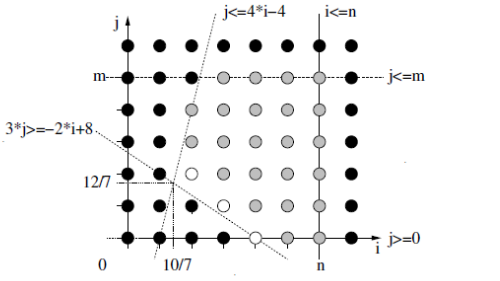
\includegraphics[width=\columnwidth]{poly.png}
%	\caption{Representación poliédrica de dos bucles anidados}
%	\label{fig:polytope_1}
%\end{figure}
%%%%%%%%%%%%%%%%%%%%%%%%%%%%%%%%%%%%%%%%%%%%%%%%%%%%%%%%%%%%%%%%%%%%%%%%%%%%%%%%%%%%%%%%%%

%La Matriz \ref{ec:matrix_1} que representa las restricciones de la serie de bucles 
%anidados en el Listado \ref{code:polycode1}, delimitará el espacio de iteraciones descrito 
%mediante un polígono regular. 
%Al tratarse en este caso de un polígono de dos dimensiones se trata de un poliedro, pero 
%en general, para espacios de iteraciones $n$-dimensionales, cuando existen $n$ 
%bucles anidados, se habla del concepto topológico de politopo.

